\chapter{Aufbau und Grundfunktionen}

Die PUMA-Einstiegsseite (~\autoref{fig:hauptmenü}) ist folgendermaßen aufgebaut:\\
1 -- \nameref{sec:suche}\\ 
2 -- \nameref{sec:spracheinstellung}\\
3 -- \nameref{sec:hauptmenue}\\
4 -- \nameref{sec:benutzermenue}\\
5 -- \nameref{sec:inhaltsbereich}\\
6 -- \nameref{sec:kontextmenue}\\ 

\begin{figure}[htb]
 \centering
 \fbox{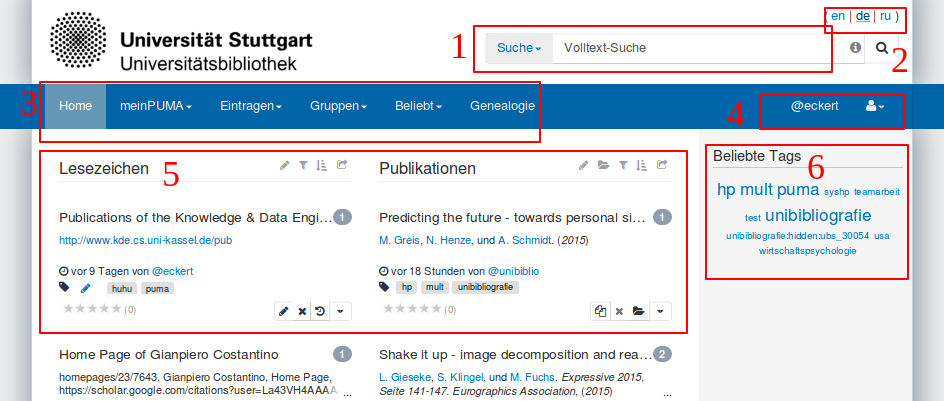
\includegraphics[width=12cm]{Bilder/Kapitel4/Puma_Hauptmenue}}
 \caption{Hauptmenü}
 \label{fig:hauptmenü}
\end{figure} 

\section{Suche}
\label{sec:suche}
Die Suche\index{Volltextsuche} (\textcolor{red}{1} in ~\autoref{fig:hauptmenü}) bietet die Möglichkeit, das System nach unterschiedlichen Kriterien zu durchsuchen. Standardmäßig werden alle Felder und Dateien durchsucht. Durch das Klicken auf das Dropdown-Menü \enquote{Suche}\index{Suche} lässt sich eingrenzen, in welchen Kategorien gesucht werden soll. Mit Hilfe von Suchsystemtags (\textit{sys:<Feldname><Feldwert>}) kann in Kategorien gezielt recherchiert werden (~\autoref{itm:suchSystemtag}).
 
\begin{figure}[h!]
 \centering
 \fbox{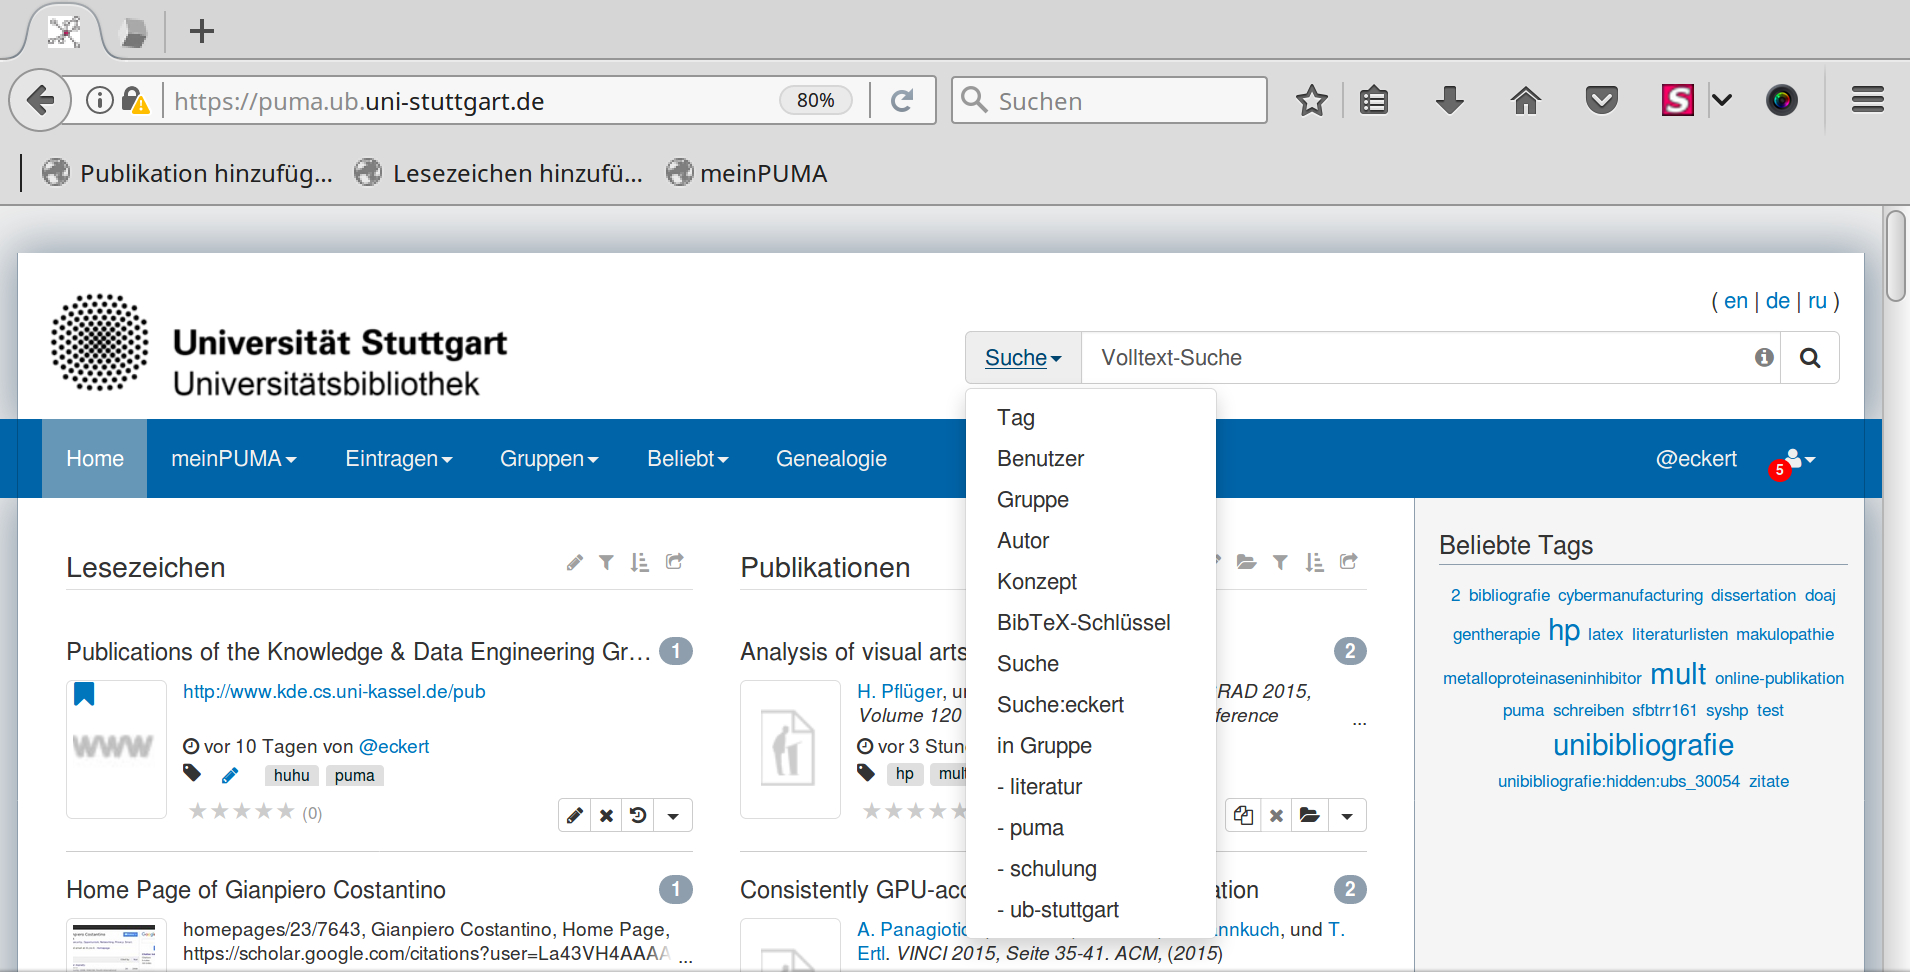
\includegraphics[width=10cm]{Bilder/Kapitel4/Suchleiste}}
 \caption{Suchleiste}
 \label{fig:suchleiste}
\end{figure} 

\section{Spracheinstellung}
\label{sec:spracheinstellung}
Die PUMA-Oberfläche kann in drei verschiedenen Sprachen (\textcolor{red}{2} in ~\autoref{fig:hauptmenü}) \index{Sprache} angezeigt werden:
Englisch (en), Deutsch (de) oder Russisch (ru)
%\begin{wrapfigure}{l}{5cm}
%\begin{mdframed}[style=tipp] \texttt{Einstellen der Standardsprache: Im Benutzermenü über den Reiter \enquote{Einstellungen} die Rubrik \enquote{Einstellungen} auswählen. Auf der erscheinenden Seite kann man die gewünschte Sprache festlegen. Die Änderung muss über \enquote{Layout speichern} bestätigt werden.}
%\end{mdframed}
\begin{tipp}
\texttt{Einstellen der Standardsprache: Im Benutzermenü über den Reiter \enquote{Einstellungen} die Rubrik \enquote{Einstellungen} auswählen. Auf der erscheinenden Seite kann man die gewünschte Sprache festlegen. Die Änderung muss über \enquote{Layout speichern} bestätigt werden.}
\end{tipp}
%\end{wrapfigure}
  

\section{Hauptmenü}
\label{sec:hauptmenue}
Nach dem Einloggen können über das Hauptmenü (\textcolor{red}{3} in ~\autoref{fig:hauptmenü}) wichtige Funktionen von PUMA ausgewählt werden:
\begin{itemize}
\item ~\nameref{subsec:home}
\item ~\nameref{subsec:meinPuma}
\item ~\nameref{subsec:eintragen}
\item ~\nameref{subsec:gruppen}
\item ~\nameref{subsec:beliebt}
\item ~\nameref{subsec:genealogie}
\end{itemize}

\subsection{Home\index{Home}}
\label{subsec:home}
Über das Menü \textit{Home} kann man jederzeit zurück auf die Startseite gelangen, auf der die neuesten Publikationen und Lesezeichen-Einträge angezeigt werden.

\subsection*{Mein PUMA\index{Mein PUMA}}
\label{subsec:meinPuma}
Mit den Standardeinstellungen \index{Funktionen!Einfache} können im Hauptmenü \textit{meinPUMA} im eingeloggten Modus folgende Untermenüs ausgewählt werden:
\begin{description}
\item [meine Einträge\index{Einträge}:] Eigenes Publikations- und Lesezeichenverzeichnis
\item [diskutierte Einträge\index{Einträge!diskutierte}:] Bewertungen von Publikationen und Lesezeichen, die selbst oder von anderen Nutzern an den eigenen Einträgen vorgenommenen wurden. 
\item [verfolgte Einträge\index{Einträge!verfolgen}:] Publikationen und Lesezeichen der Nutzer, denen man folgt (~\autoref{}) 
\item [Einträge von Freunden\index{Einträge!von Freunden}:] Einträge der befreundeten Nutzer werden angezeigt (~\autoref{}).
\end{description}
Im Benutzermenü können über \textit{Einstellungen} $\to$ Reiter \textit{Einstellungen} erweiterte Funktionen\index{Funktionen!Erweiterte} eingestellt werden. Das Menü wird um folgende Funktionen ergänzt:
\begin{description}
\item [private Einträge\index{Einträge!privat}:] Publikationen und Lesezeichen, die nur im eigenen Nutzerkonto sichtbar sind. 
\item [Einträge für Freunde\index{Einträge!Freunde}:] Einträge, die auch mit den befreundeten Nutzer geteilt werden.
\item [Dokumente\index{Dokumente}:] Übersicht über die angehängten Dokumente
\item [Duplikate\index{Duplikate}:] zeigt doppelte Einträge im eigenen Konto an
\item Konzepte\index{Konzepte}:] Anzeige angelegter Konzepte (Gruppe von Schlagwörtern unter einem Supertag) (~\autoref{}). 
\item [Lebenslauf\index{Lebenslauf}:] Hier können persönliche Daten hinterlegt werden, die für andere Nutzer in PUMA sichtbar sind.
\item [Publikationen durchstöbern:] Mit dieser Funktion können eigene Lesezeichen und Publikationen dynamisch durch Auswahl von \tags und Autoren-Listen durchsucht werden. Zusätzlich gibt es Auswahl-Buttons für UND- oder ODER-Verknüpfungen.
\item [BibTex\index{BibTex} exportieren:] Exportiert alle Publikationen in der eigene Sammlung im BibTex-Format.
\end{description}

\subsection{Eintragen}
\label{subsec:eintragen}
\begin{description}
    \item [Lesezeichen hinzufügen\index{Lesezeichen!eintragen}:] Ein neues Lesezeichen der eigenen Sammlung hinzufügen.  
    \item [Publikation hinzufügen\index{Publikationen!eintragen}:] Eine neue Publikation der eigenen Sammlung hinzufügen. 
    \item [Lesezeichen importieren\index{Lesezeichen!Import}:] Lesezeichen aus dem Browser oder Delicious (~\autoref{}) importieren.
    \item [Publikationen importieren\index{Publikationen!Import}:] Bestehende BibTeX- oder EndNote-Datei importieren.
\end{description}

\subsection{Gruppen}
\label{subsec:gruppen}
Zeigt Funktionen zu Gruppen\index{Gruppen} an sowie die Gruppen in denen man Mitglied ist.
\begin{description}
    \item [Alle Gruppen:] Überblick über alle existierenden Gruppen bei PUMA
    \item [Eine neue Gruppe erstellen:] eine eigene Gruppe kann erstellt werden (~\autoref{})
\end{description}
\subsection{Beliebt\index{Beliebt}}
\label{subsec:beliebt}
Die drei häufigsten Einträge der letzten 7, 30 bzw. 120 Tage werden angezeigt.
\begin{description}
    \item [Einträge:] Zeigt die beliebtesten Einträge an.
    \item [\tags:] Zeigt die beliebtesten \tags in einer Schlagwortwolke an. Je größer ein \tag ist, desto häufiger wird dieser verwendet.
    \item [Autor:] Zeigt die beliebtesten Autoren an.
    \item [Konzepte:] Zeigt die beliebtesten Konzepte und deren Zuordnungen an. 
    \item [Diskussionen:] Zeigt Lesezeichen und Publikationen an, über welche viel diskutiert wurde. 
\end{description}
\subsection{Genealogie}
\label{subsec:genealogie}
Die PUMA Genealogie \href{https://www.uni-kassel.de/fb07/index.php?id=38090}{https://www.uni-kassel.de/fb07/index.php?id=38090} hat zum Ziel, einen Stammbaum der Forschung an deutschen Universitäten aufzubauen. Die Ausgangspunkt ist der Dissertationskatalog der Deutschen Nationalbibliothek. Nutzer haben die Möglichkeit, ihre betreuten Arbeiten mit ihrem Namen zu verknüpfen. Diese Funktion wird zwar in PUMA angezeigt, bisher aber nicht aktiv mit Daten gepflegt.

\section{Benutzermenü}
\label{sec:benutzermenue}
\subsection{@username\index{@username}}
\label{subsec:username}
Eigenes Publikations- und Lesezeichenverzeichnis
\subsection{Das Personensymbol}
\label{subsec:Personensymbol}
\begin{description}
\item[Eingang\index{Eingang}:] Nutzer, mit denen man befreundet ist oder den gleichen Gruppen angehört, können sich Publikationen und Lesezeichen zuschicken (\tag \textit{send:Benutzername}). Diese Einträge werden im Eingang angezeigt (\tag \textit{sent:Benutzername}) und können in die eigene Sammlung übernommen werden.
\item [Ablage\index{Ablage}:] In der Ablage können Literaturlisten zusammengestellt werden. Diese Listen können exportiert werden oder die Einträge gesammelt bearbeitet werden (~\autoref{}). 
\item [Freunde\index{Freunde}:] Überblick über die Nutzer, die als Freund hinzugefügt wurden 
\item [Tags bearbeiten\index{Tags!bearbeiten}:] \tags und Konzepte bearbeiten: Es können beispielsweise \tags durch neue in einer Stapelverarbeitung ersetzt werden (~\autoref{}).
\item [Einstellungen\index{Einstellungen}:] Zeigt persönlichen Benutzereinstellungen an. Hier kann das Profil eingestellt, die allgemeine Einstellungen, den Lebenslauf sowie Einstellungen zu Gruppen geändert werden.
\item [Weblog\index{Weblog}:] Leitet zum Blog der UB Stuttgart weiter. Hier werden Neuigkeiten zu \footnote{\url{http://blog.ub.uni-stuttgart.de/category/puma/}} PUMA veröffentlicht.
\item [Hilfe\index{Hilfe}:] Online-PUMA-Hilfe.
\item [Abmelden\index{Abmelden}:] Logout 
\end{description}

\section{Inhaltsbereich}
\label{sec:inhaltsbereich}
Hier werden die öffentlich  geteilten Lesezeichen und Publikationen aller Nutzern angezeigt. Dir neusten Einträge erscheinen oben.
\section{Kontextmenü}
\label{sec:kontextmenue}
Auf der Einstiegsseite werden die beliebtesten Tags\index{Tags} angezeigt. In den Einstellungen kann zwischen der Wolken- oder Listen-Ansicht gewählt werden.
\newpage
\section{Der PUMA-Aufbau im Überblick}
\label{sec:pumaAufbau}
%\small

\tabulinesep=1.5mm
\begin{longtabu}{|X[l]|X[l]|X[l]|}\hline
\rowfont\bfseries
Hauptmenü & Untermenü & Rubrik \\  \hline
\endfirsthead
\hline
%\multicolumn{4}{@{}l}{\small\dots\emph{Fortsetzung}}\\ \hline
\rowfont\bfseries
Hauptmenü & Untermenü & Rubrik \\  \hline
\endhead
\hline
%\multicolumn{4}{@{}l}{\small\dots\emph{Fortsetzung nächste Seite} \ldots}\\ \hline
\endfoot
%\hline
\endlastfoot
Eintragen&Lesezeichen hinzufügen &- \\ \cline{2-3}
&Publikation hinzufügen &Dokument hochladen \\ \cline{3-3}
&&BibTex/EndNote-Schnipsel\\ \cline{3-3}
&&Code scannen \\\cline{3-3}
&&Per Hand\\ \cline{2-3}
&Lesezeichen importieren&- \\ \cline{2-3}
&Publikationen importieren &-\\ \hline
Gruppen&Alle Gruppen& Gruppen von A-Z\\ \cline{2-3}
&Gruppen, in denen Nutzer Mitglied sind& Einträge\\\cline{3-3}
&&Interessant für  \\ \cline{3-3}
&&Sichtbar\\ \cline{3-3}
&&Dokumente\\ \cline{3-3}
&&diskutierte Einträge\\ \cline{3-3}
&&Einstellungen\\ \cline{2-3}
&Eine neue Gruppe erstellen&-\\ \hline
Personensymbol&Eingang&-\\ \cline{2-3}
&Ablage&-\\ \cline{2-3}
&Freunde&Ihre Freunde \\ \cline{3-3}
&&Sie sind ein Freund von \\ \cline{2-3}
&Tags bearbeiten&-\\ \cline{2-3}
&Einstellungen&Mein Profil\\ \cline{3-3}
&&Einstellungen\\ \cline{3-3}
&&JabRef Layout-Datei\\\cline{3-3}
&&Lebenslauf\\ \cline{3-3}
&&OAuth-Consumers \\\cline{3-3}
&&Gruppen\\\cline{3-3}
&&Synchronisation\\\cline{2-3}
&Weblog&-\\\cline{2-3}
&Hilfe&-\\\cline{2-3}
&Abmelden&-\\\hline
\caption{Der PUMA-Aufbau im Überblick}
\label{tab:pumaAufbau}
\end{longtabu}

%\normalsize

